\chapter{Configuration \& Business Logic}

\section*{Module Configuration}

\subsection*{Coffee Outlet}
Each coffee outlet has a digital record in the ERP. Key configurations include:
\begin{itemize}
    \item \textbf{Outlet Name:} The unique identifier of the branch.
    \item \textbf{Location:} Physical address used for reporting and mapping.
    \item \textbf{Manager:} Linked to an employee in the system.
    \item \textbf{Integration with Sales:} Outlets are associated with each sales order for proper reporting and revenue tracking.
\end{itemize}

\subsection*{Coffee Menu Items}
The menu module defines all items sold in outlets. Configuration fields include:
\begin{itemize}
    \item \textbf{Name:} The item name (required).
    \item \textbf{Price:} Set in the company currency; used in sales orders.
    \item \textbf{Category:} Drinks, Snacks, Desserts, or Vegan.
    \item \textbf{Status:} Draft, Active, Seasonal, or Retired.
    \item \textbf{Image:} Optional image for kanban or POS display.
    \item \textbf{Customization Options:} Milk type, size, syrup flavor, and extra shot.
    \item \textbf{Linked Product:} Each menu item automatically creates/updates a `product.product` record for integration with the sales and accounting modules.
\end{itemize}

\subsection*{Access Control}
\begin{itemize}
    \item Users with the \texttt{access\_coffee\_menu\_item\_user} or \texttt{access\_coffee\_menu\_tag\_user} groups can create, read, write, and delete menu items or tags.
    \item Manager-level permissions can be configured in Odoo's security groups for outlets and sales.
\end{itemize}



\section*{Business Logic}

\subsection*{Menu Item Lifecycle}
\begin{itemize}
    \item When a menu item is created, the system automatically generates a linked product in the Odoo product catalog.
    \item Updates to price, name, or category propagate to the linked product.
    \item Deleting or retiring a menu item ensures it is no longer selectable in sales transactions.
\end{itemize}

\subsection*{Sales Order Integration}
\begin{itemize}
    \item Each sales order references the outlet (`coffee.outlet`) and customer (`res.partner`) directly.
    \item Items added to the order are linked to the `product.product` created by the menu module.
    \item This ensures correct pricing and consistency between menu configuration and sales transactions.
\end{itemize}

\subsection*{Customization Handling}
\begin{itemize}
    \item Customer preferences (milk type, size, syrup flavor, extra shot) are stored per order line.
    \item These preferences do not create new products but are saved in order notes for outlet preparation.
\end{itemize}

\subsection*{Tagging Logic}
\begin{itemize}
    \item Menu items can be assigned tags (`coffee.menu.tag`) for categorization or filtering in POS and reports.
    \item Tags are independent and reusable across multiple items.
\end{itemize}

\section*{Recommended Diagrams}
\begin{itemize}
    \item \textbf{Flow Diagram:} Shows the creation of a menu item and automatic product linkage.
    \item \textbf{Sequence Diagram:} Illustrates a sales order being placed, linking outlet, customer, and menu item.
\end{itemize}

\begin{figure}[H]
\centering
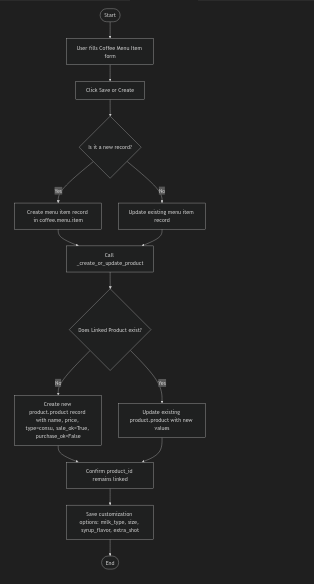
\includegraphics[width=0.6\textwidth,keepaspectratio]{diagrams/flowdiagram.png}
\caption{Flow Diagram: Menu Item Creation and Product Linkage}
\end{figure}

\begin{figure}[H]
\centering
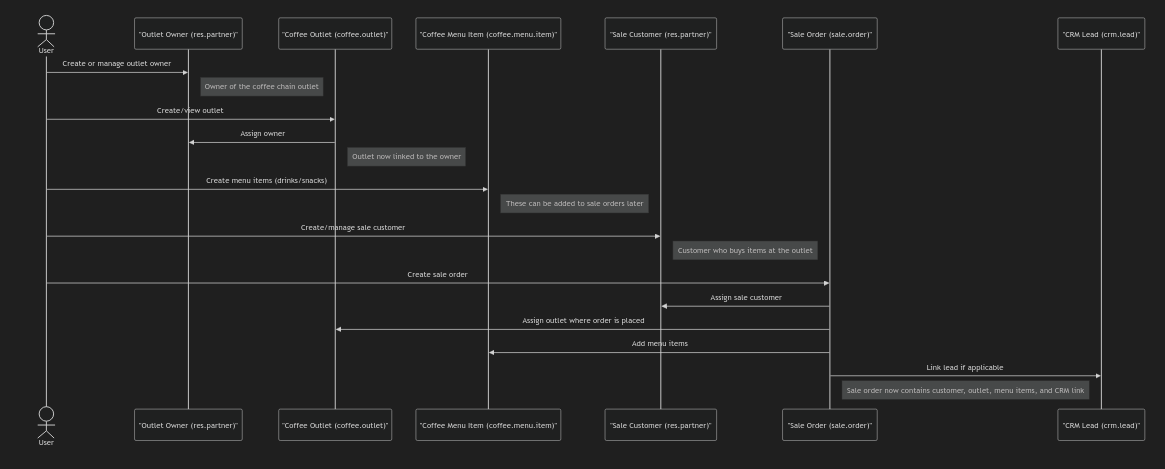
\includegraphics[width=1.0\textwidth,keepaspectratio]{diagrams/sequence.png}
\caption{Sequence Diagram: Sales Order Processing in Coffee Chain ERP}
\end{figure}
